\documentclass[a4paper,11pt]{article}
\usepackage{amsmath,amsthm,amsfonts,amssymb,amscd,amstext,vmargin,graphics,graphicx,tabularx,multicol} \usepackage[french]{babel}
\usepackage[utf8]{inputenc}  
\usepackage[T1]{fontenc} 
\usepackage[T1]{fontenc}
\usepackage{amsmath,amssymb}
\usepackage{pstricks-add,tikz,tkz-tab,variations}
\usepackage[autolanguage,np]{numprint} 
\usepackage{color}
\usepackage{ulem}

\setmarginsrb{1.5cm}{0.5cm}{1cm}{0.5cm}{0cm}{0cm}{0cm}{0cm} %Gauche, haut, droite, haut
\newcounter{numexo}
\newcommand{\exo}[1]{\stepcounter{numexo}\noindent{\bf Exercice~\thenumexo} : \marginpar{\hfill /#1}}
\reversemarginpar


\newcounter{enumtabi}
\newcounter{enumtaba}
\newcommand{\q}{\stepcounter{enumtabi} \theenumtabi.  }
\newcommand{\qa}{\stepcounter{enumtaba} (\alph{enumtaba}) }
\newcommand{\initq}{\setcounter{enumtabi}{0}}
\newcommand{\initqa}{\setcounter{enumtaba}{0}}

\newcommand{\be}{\begin{enumerate}}
\newcommand{\ee}{\end{enumerate}}
\newcommand{\bi}{\begin{itemize}}
\newcommand{\ei}{\end{itemize}}
\newcommand{\bp}{\begin{pspicture*}}
\newcommand{\ep}{\end{pspicture*}}
\newcommand{\bt}{\begin{tabular}}
\newcommand{\et}{\end{tabular}}
\renewcommand{\tabularxcolumn}[1]{>{\centering}m{#1}} %(colonne m{} centrée, au lieu de p par défault) 
\newcommand{\tnl}{\tabularnewline}

\newcommand{\trait}{\noindent \rule{\linewidth}{0.2mm}}
\newcommand{\hs}[1]{\hspace{#1}}
\newcommand{\vs}[1]{\vspace{#1}}

\newcommand{\N}{\mathbb{N}}
\newcommand{\Z}{\mathbb{Z}}
\newcommand{\R}{\mathbb{R}}
\newcommand{\C}{\mathbb{C}}
\newcommand{\Dcal}{\mathcal{D}}
\newcommand{\Ccal}{\mathcal{C}}
\newcommand{\mc}{\mathcal}

\newcommand{\vect}[1]{\overrightarrow{#1}}
\newcommand{\ds}{\displaystyle}
\newcommand{\eq}{\quad \Leftrightarrow \quad}
\newcommand{\vecti}{\vec{\imath}}
\newcommand{\vectj}{\vec{\jmath}}
\newcommand{\Oij}{(O;\vec{\imath}, \vec{\jmath})}
\newcommand{\OIJ}{(O;I,J)}

\newcommand{\bmul}[1]{\begin{multicols}{#1}}
\newcommand{\emul}{\end{multicols}}


\newcommand{\reponse}[1][1]{%
\multido{}{#1}{\makebox[\linewidth]{\rule[0pt]{0pt}{20pt}\dotfill}
}}

\newcommand{\titre}[5] 
% #1: titre #2: haut gauche #3: bas gauche #4: haut droite #5: bas droite
{
\noindent #2 \hfill #4 \\
#3 \hfill #5

\vspace{-1.6cm}

\begin{center}\rule{6cm}{0.5mm}\end{center}
\vspace{0.2cm}
\begin{center}{\large{\textbf{#1}}}\end{center}
\begin{center}\rule{6cm}{0.5mm}\end{center}
}



\begin{document}
\pagestyle{empty}
\titre{ Interrogation : Fonction linéaire}{Nom}{Prénom}{Date}{Classe}





\exo{2} Les fonctions suivantes sont-elles linéaires ? Si oui, précisez leur coefficient.

\bmul{4}

$ f : x \longmapsto 6x - 1$ \\

$ j : x \longmapsto -\dfrac{2}{7}x$ \\

\columnbreak

$ g : x \longmapsto \dfrac{x}{5}$ \\

$ k : x \longmapsto 5x-3,2x$ \\

\columnbreak

$ h : x \longmapsto -3x^{2}$ \\

$ m : x \longmapsto -x$ \\

\columnbreak

$ i : x \longmapsto \dfrac{5}{x}$ \\

$ n : x \longmapsto -3(x-2)$ \\

\emul

\noindent \reponse[6]\\


\vspace*{0.5cm}

\exo{1} \\
$f$ est une fonction linéaire telle que $f(7) = -2$. \textbf{Sans déterminer le coefficient de f}, calculer : \\

\qa l'image de 21 ?\\ 
\reponse[2]\\

\qa l'image de 3,5 ?\\
\reponse[2]\\

\vspace*{0.5cm}


\exo{3} Durant les soldes, un magasin pratique une remise de 35 $\%$ sur tous les articles.\\

\q Soit $f$ la fonction linéaire qui permet de transformer le prix initial $x$ en prix soldé $f(x)$. \\
\textbf{Donner l'expression de la fonction $f$}.\\
\reponse[2]\\

\q Quelle est l'image de 125 par la fonction $f$ ? (Écrire vos calculs)\\
\reponse[2]\\


\q Quel est l'antécédent de 29,90 par la fonction $f$ ? (Écrire vos calculs)\\
\reponse[2]\\



\newpage

\exo{1.5} Voici les représentations graphiques respectives de trois
fonctions $g$, $k$ et $d$.

\begin{center}
\includegraphics[scale=0.8]{graph2interro.eps} 
\end{center}

\initq \q Parmi les représentations graphiques ci-dessus, lesquelles sont celles de fonctions linéaires ? Justifier votre réponse.\\
\reponse[2]\\

\q Quelle est l'image de 4 par la fonction $g$ ? Quelle est l'image de -1 par la fonction $g$ ? \\
\reponse[1]\\

\q Grâce à la représentation graphique, donner l'expression algébrique de la fonction $g$. \\
\reponse[1]\\




\exo{2.5}
Tracer la représentation graphique de chaque fonction dans les repères suivants :

\begin{center}
\includegraphics[scale=0.85]{graphinterro.eps} 
\end{center}

\newpage





\end{document}
